\chapter{序論}
\label{chap:introduction}

\section{背景}
\label{section:background}
高齢化社会の中でひとり暮らしの高齢者が多くなっている。
その中でも糖尿病を患っている人は、他人の監視の目もなく自分で薬物療法などによって治療を行っている。
一人暮らしの中薬の用法容量を守って摂取していくためには習慣化が必須で、最初は特に継続していくのが難しい。

\subsection{糖尿病について}
\label{subsection:diabetes}

糖尿病とは、膵臓から分泌されるホルモンであるインスリンが十分に働かない、もしくは十分に分泌されないことによって、血液中を流れるブドウ糖(血糖)が増えてしまう病気である。\cite{diabetes}
インスリンは元来、血糖を一定の範囲に抑える働きを担っており、これが不足してしまうことは身体機能として異常をきたしていることになる。
血糖値が高い状態が何年も続くことで血管が傷つき、将来的に心臓病、失明、腎不全、足の切断などのより重い病気に繋がる可能性もある。(慢性合併症)

我々が食事をすると、栄養素の一部は等となって腸から吸収される。そして長時間食事をしない時間が続くときには、主に肝臓により食べたものが糖に変換されている。
糖は人間の体のエネルギー源であり、血液中を流れ筋肉にたどり着いた糖はインスリンの力を借りて初めて、細胞に取り込まれ、実際に体を動かすことに使用される。
糖がそうして血中から細胞に取り込まれることで血液中の糖分濃度は徐々に一定に戻っていく。
すなわち、インスリンは糖を体のエネルギーとして使うために必須と言えるホルモンなのである。\cite{diabetes}

糖尿病における、インスリンが十分に働かない原因は2種類に分類される。\cite{diabetes}

\begin{description}
  \item [インスリン分泌低下]\mbox{}\\
    膵臓の機能の低下により、十分なインスリンを作れず分泌量が少なくなる状態。血中に流れている糖の量に対して細胞に取り込むためのインスリンが足りないため、血液中に糖があふれてしまう。
  \item [インスリン抵抗性]\mbox{}\\
    インスリンは十分な量が作られているが、その効果を発揮できない状態。運動不足や食べ過ぎが原因で肥満になると、インスリンが働きにくくなる。よって細胞内に糖が十分に取り込まれず、血液中に糖があふれてしまう。
\end{description}

糖尿病にはその原因別にいくつか種類があるが、大きく分けると「1型糖尿病」、「2型糖尿病」、「その他の特定の機序、疾患によるもの」、そして「妊娠糖尿病」が存在する。\cite{diabetes}

\begin{description}
  \item [1型糖尿病]\mbox{}\\
    上記にあげたインスリン分泌低下により血糖値が高いままになってしまうもの。生きるために、注射でインスリンを補う治療が必須になる。そして、この状態をインスリン依存状態と呼ぶ。
  \item [2型糖尿病]\mbox{}\\
    上記にあげたインスリン分泌低下、もしくはインスリン抵抗性が強くなることで血糖値が高いままになってしまうもの。原因としては、遺伝、過食、運動不足、肥満など環境的な影響や生活習慣の影響が大きいた言われている。
    多くの患者は食事や運動習慣の見直しから始め、必要に応じて飲み薬やインスリン注射などで治療を行う。
  \item [その他の特定の機序、疾患によるもの]\mbox{}\\
    糖尿病以外の疾患などにより血糖値が上昇し、結果として糖尿病を発症してしまうケース
  \item [妊娠糖尿病]\mbox{}\\
    妊娠中に初めて発覚した血糖の上昇のこと。(糖尿病ではない)胎盤から出るホルモンの影響で妊娠中はインスリン抵抗性が強くなり、食後の血糖値が上昇しやすくなる。
\end{description}

本論文では、上記にあげた糖尿病患者の中でも、インスリン分泌低下、もしくはインスリン抵抗性が高まったためにインスリン注射を必要とする患者を対象とする。

現在の日本において、糖尿病患者の数は実に約328万9千人とされ、治療を必要とする人間が多く存在する。\cite{diabetes_statistics}
糖尿病は適度な運動を定期的に行っていなかったり、食生活が偏っていることが理由としてあげられる。(ここで糖尿病が上昇傾向にある理由のリファレンスをつける。)

\begin{figure}[htbp]
  \caption{近年における糖尿病患者数の推移(文献\cite{diabetes_statistics}より引用)}
  \label{fig:diabetes_total_number}
  \begin{center}
    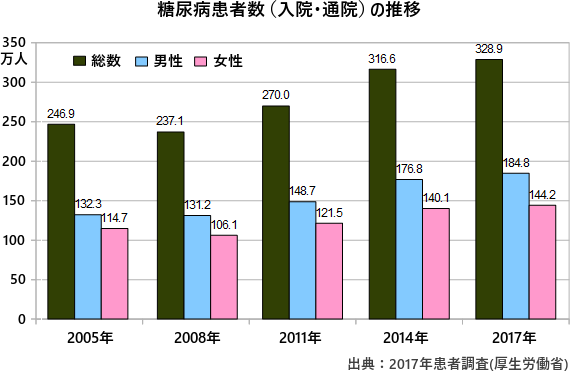
\includegraphics[bb=0 0 900 400,width=25cm]{assets/diabetes_total_number.png}
  \end{center}
\end{figure}

図\ref{fig:diabetes_total_number}は、国勢調査で実際に観測された糖尿病患者数を表している。横軸が左から右へ2005年、2008年となっていることから、この調査は3年に1度行われていることが見て取れ、
その糖尿病患者数は、2005年から毎回上昇していることがわかる。

糖尿病の治療方法としては、運動療法、食事療法、薬物療法が挙げられるが、厚生労働省も掲げる通り、「1に運動2に食事、最後に薬」と言われている。

65歳以上の患者数が最多になっていること。

独居老人はどれくらい?独居老人の中で糖尿病を患っている人は?

\newpage

\subsubsection{糖尿病におけるインスリン治療について}
\label{subsubsection:insulin_treatment}

インスリン治療は、主にインスリン依存状態に陥る糖尿病1型患者、また、症状や進行状況によっては2型糖尿病患者も行う治療方法である。\cite{insulin_treatment_method}

糖尿病を患っていない健康な人、軽い糖尿病の人、思い糖尿病の人それぞれのの血糖値推移を図\ref{fig:suger_in_blood_change}に示す。
一般に、健康な人は1日を通して血糖値140mgを超えない範囲で推移するが、糖尿病患者は200mgを超える高血糖状態が続いている。

\begin{figure}[htbp]
  \caption{1日の血糖値の変化(文献\cite{suger_in_blood_change}より引用)}
  \label{fig:suger_in_blood_change}
  \begin{center}
    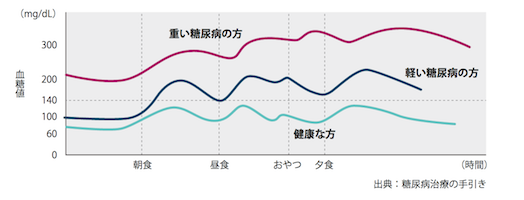
\includegraphics[bb=0 0 500 200,width=15cm]{assets/suger_in_blood_change.png}
  \end{center}
\end{figure}

インスリン療法は、糖尿病患者の血糖値の推移を、図\ref{fig:suger_in_bloock_change}に示したような健常者の血糖値推移に限りなく近づけることを目標に、適切なタイミングに適切な量投与する手法である。

その注射の頻度と、容量は患者によって様々であるが、一般的に用いられるのは毎食前3回と就寝前1回の計4回の4回法と呼ばれる治療法である。\cite{insulin_treatment_method}\cite{diabetes_treatment_type1}
専用の注射器を使い下腹部に自分で直接インスリンを注入するものだ。これにより体内に足りない、もしくは抵抗性が強くなっているインスリンをに対して追加でインスリンを取り込み、
食事後に起こる血糖値の上昇を一定に抑え、常に血糖値が高くなってしまう状況を回避する。

\newpage

図\ref{fig:insulin_4times_method}に4回法の注射タイミングを示す。

\begin{figure}[htbp]
  \caption{インスリン療法、4回法の具体例(文献\cite{insulin_4times_method}より引用)}
  \label{fig:insulin_4times_method}
  \begin{center}
    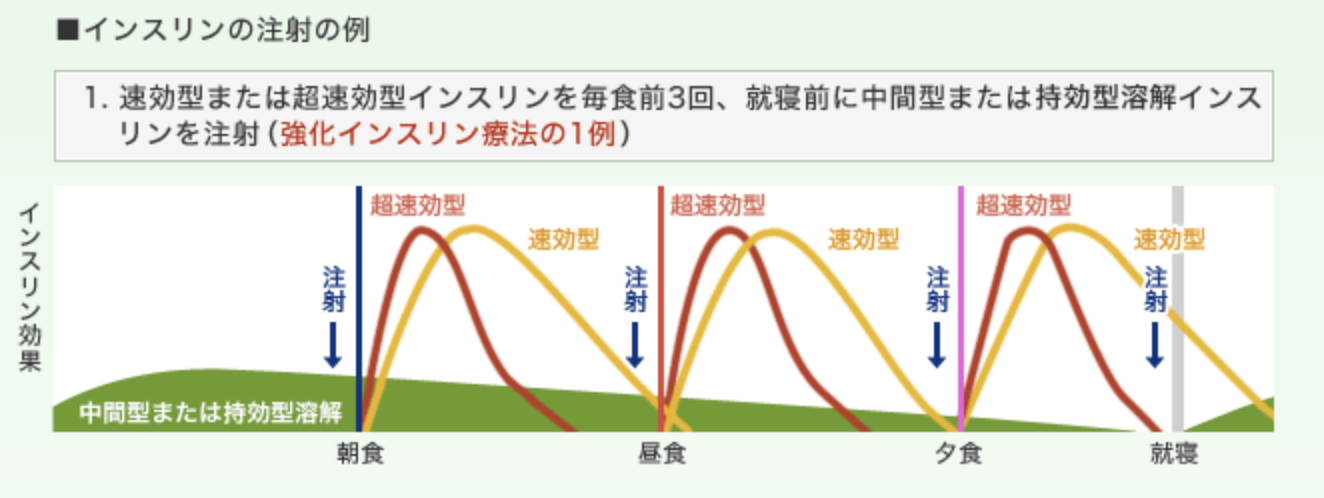
\includegraphics[bb=0 0 700 300,width=15cm]{assets/insulin_4times_method.png}
  \end{center}
\end{figure}

\paragraph{インスリン注射の手順}
\label{paragraph:insulin_injection_steps}

インスリンを服薬する際の手順を以下に示す。
インスリン注射には図\ref{fig:insulin_pen_needle}に示すような注射器(奥)と針(手前)を使用する。

\begin{enumerate}
  \item インスリンの注射の針を開封し注射器に装着する。
  \item 一度注射器の端のメモリをある程度回転させ、注射器の中の空気を押し出す。
  \item 医師に指示を受けている分摂取できるよう注射器の端をねじり、調整する。
  \item 針を刺す下腹部の表面をを消毒し、注射器を刺し、注射器の反対側の端を親指でゆっくり押していく。
  \item 押し切って5秒ほど静止したのち、ゆっくりと針を抜く。
\end{enumerate}

\begin{figure}[htbp]
  \caption{インスリン注射器と針}
  \label{fig:insulin_pen_needle}
  \begin{center}
    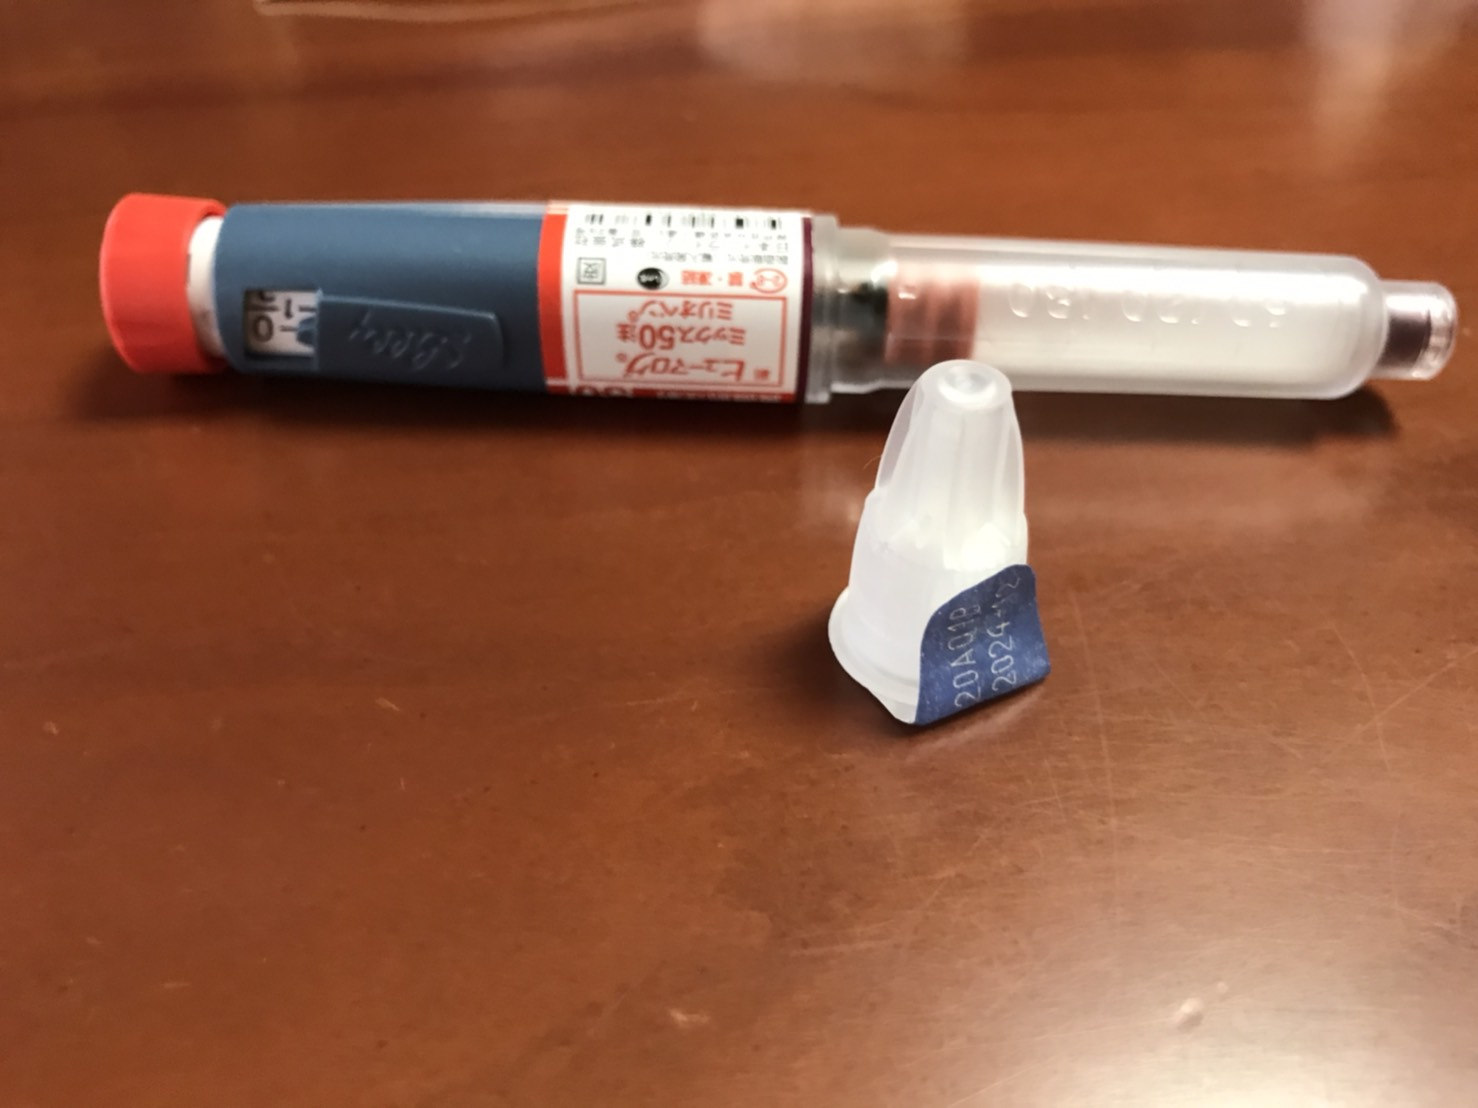
\includegraphics[bb=0 0 1300 1200,width=10cm]{assets/insulin_pen_needle.jpg}
  \end{center}
\end{figure}

\newpage

\subsection{一般的な薬物療法について}
\label{subsection:drug_treatment}

ここから一般的な薬物療法に関する課題点の背景を述べる。

一般に、医者から処方された薬を、用法要領を守って服薬し続けることが難しいというアンケート調査結果が図\ref{fig:forget_medicine_number}に示されている。

\begin{figure}[htbp]
  \caption{処方薬の飲み残しに関する意識・実際調査の結果(文献\cite{drug_treatment_investigation}より引用)}
  \label{fig:forget_medicine_number}
  \begin{center}
    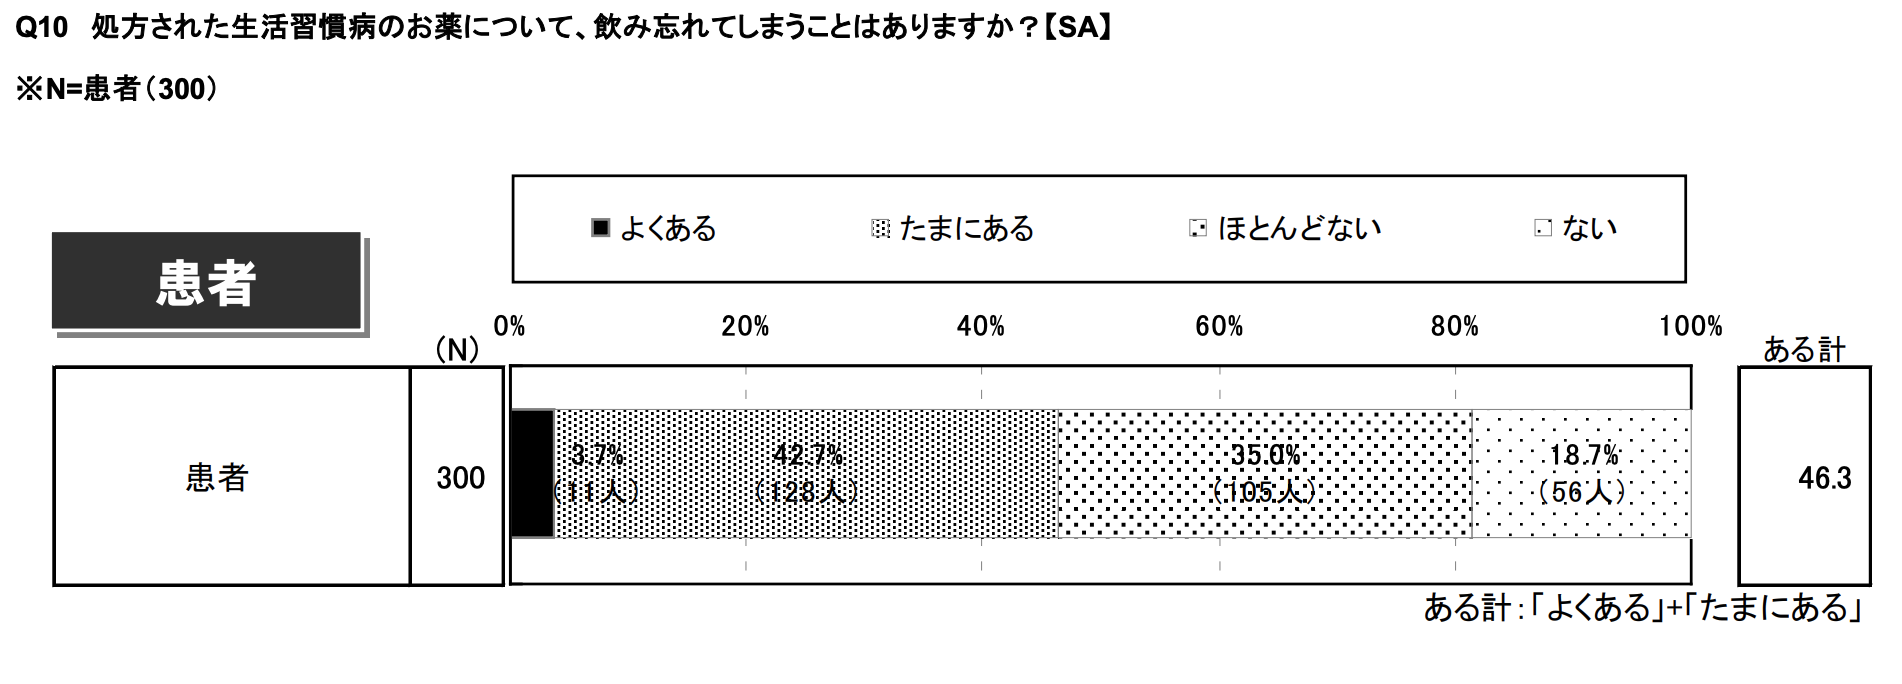
\includegraphics[bb=0 0 1000 400,width=15cm]{assets/forget_medicine_number.png}
  \end{center}
\end{figure}

実際に図\ref{fig:forget_medicine_number}のアンケート結果を見てみると、○%ほどの人が処方された薬を服薬し忘れる傾向があることがわかる。また、この調査は高血圧、高脂血症、糖尿病のいづれかで現在通院中の上、処方薬を使用している生活習慣病の患者を対象にしている\cite{drug_treatment_investigation}ため、本研究で対象としている糖尿病患者も含まれており、薬物治療において服用し忘れが起こる可能性を示唆している。
先ほども\ref{subsection:diabetes}で述べたように、一般的な糖尿病治療の薬の服薬タイミングは厳密に決まっており、毎食前3回と睡眠前1回、インスリンを直接下腹あたりに直接注射することで服用が完了するが、これを忘れると血糖値が上昇したままになってしまうので、糖尿病患者にとってインスリン摂取を忘れることは避けたいものである。

\subsection{問題意識・対象}

どんな人を対象とするのか、どんな食事内容なのか詳細に書く。

\section{本研究で解決したい問題}
\label{section:problem}

本論文では、食前のインスリン注射を服用し忘れてしまい、それに気づかないまま食事を行ってしまう患者に対して、忘れていることを知らせる手段がない問題を解決することを目指す。
現在の治療方法では、患者自身の自己管理能力や、その周りの監視の目に依存してしまっている。
結果として、もし服用を忘れたとしても、それに気づくことなく生活してしまった場合、体調悪化、最悪の場合には合併症を引き起こす可能性もある。
万が一、服用を忘れてしまった場合は、担当医に連絡を取り、状況を説明、そして適切な対処を行うのが一般的である。

\section{目的}
\label{section:purpose}

本研究は、食事前にインスリン注射を服用し忘れたことを治療患者に知らせることを目的としている。
インスリン注射の服用忘れ帽子に関しては、タイマーで時限式に知らせるデバイスがプロダクトとして存在しているが、実際の食事時間が日々異なる可能性を考えると、食事前に服用を行わなければいけない患者にとっての解決策にはならない。
また、食事の検知にはカメラ映像と画像認識技術を使用した研究があるが、被験者にとって常に撮影されているという煩わしさは、実際の導入を考えると現実的ではない。
他にも、顎や腕に直接装着する形のウェアラブルデバイスを用いた食事検知の研究がなされているが、こちらも常に体に装着しておかなければならないことは同じく煩わしさに繋がる。
一方で、本研究では、画像もウェアラブルデバイスも使用せず、食事検知を行うため、以上のような煩わしさはない。

\section{本論文の構成}
\label{section:structure}
本論文における以降の構成は次の通りである。
\ref{chap:related_works}章では、本論文に関連する研究やプロダクトを紹介し、それぞれの特徴とそれらと本研究との差異を示す。
インスリンデバイス、加速度による行動検知、そして食事開始の検知と、幅広く関連研究を挙げている。
\ref{chap:design}章では、加速度センサーによる食事検知とインスリンデバイスによるインスリン摂取忘れを通知するためのシステムの設計について述べる。
\ref{chap:implementation}章では、\ref{chap:design}章で述べた内容の実装に用いたライブラリや実モジュールに言及しながら詳細な実装内容について述べる。
\ref{chap:evaluation}章では、\ref{chap:implementation}章で実装したインスリン摂取忘れ通知システムの評価を行い、その結果について考察する。
\ref{chap:conclusion}章では、本論文のまとめと今後の展望について述べる。
